\documentclass{beamer}
\usetheme{Boadilla}
\usepackage[spanish]{babel}
\usepackage{amsfonts,amssymb,amsmath,amsthm,
            amssymb,amsopn,amsxtra,amstext,amsbsy}
\usepackage{subfig} % To add subfigures
%% \usepackage{graphicx}
\usepackage{epsfig}
\usepackage{array}
\usepackage{url}
\usepackage[spanish]{babel}
\usepackage{color}
%\usepackage{float}
\usepackage{savesym}
\savesymbol{AND}
\usepackage{algorithm}
\usepackage{algorithmic}
\usepackage{enumerate}
\newtheorem*{myteo}{Teorema}
\newtheorem*{mydef}{Definici\'on}
\renewcommand{\algorithmicrequire}{\textbf{Input:}}
\renewcommand{\algorithmicensure}{\textbf{Output:}}
\def\R{{\mathbb R }}
\def\N{{\mathbb N }}

\newenvironment<>{problock}[1]{%
  \begin{actionenv}#2%
      \def\insertblocktitle{#1}%
      \par%
      \mode<presentation>{%
        \setbeamercolor{block title}{fg=white,bg=green!30!black}
       \setbeamercolor{block body}{fg=black,bg=green!7}
       \setbeamercolor{itemize item}{fg=orange!20!black}
       \setbeamertemplate{itemize item}[triangle]
     }%
      \usebeamertemplate{block begin}}
    {\par\usebeamertemplate{block end}\end{actionenv}}
\usepackage{arydshln}


\title[An Online VEC]{An Online  Vector error correction model for forecasting exchange rates}
  
\author[P. Arce]{Paola Arce \inst{1} \and Werner Kristjanpoller \inst{2} \and Luis Salinas \inst{1,3} } 
\institute[USM]{\inst{1} Departamento de Inform\'atica, UTFSM \and %
                     \inst{2} Departamento de Industrias, UTFSM \and 
                     \inst{3} CCTVal, UTFSM}
\date{\today}

\begin{document}

\frame{\titlepage}

\section[Outline]{}
\frame{\tableofcontents}

\section{Introduction}
%\subsection{Overview of the Beamer Class}

\frame{
\frametitle{Introduction}

In finance, it is common to find variables with a long-run equilibrium
relationship and also high frequency relationship which avoid arbitrage 
opportunities \footnote{Arbitrage is taking
advantage of the price differences in different markets}.  In general, 
it is believed that some set of variables cannot wander too far away from each other. 
This relationship is called {\color{blue} cointegration}.
Cointegration means that one or more combinations of these variables is stationary even
though individually they are not.
\newline
\newline
Some financial models such as {\color{blue}VEC} (vector error
correction) takes advantage of this property and describes the joint
behaviour of several cointegrated financial instruments.


%This implies cointegration between the prices of the same asset
%trading on different markets or between spot and future and forward
%prices or bid and ask prices, for example.

}


\frame{
\frametitle{Cointegration}

\begin{alertblock}{Cointegration}
A set of I(1) variables is called cointegrated if exists a linear combination of them which is I(0).
\end{alertblock}

Let $\{\mathbf{y}^1, \dots, \mathbf{y}^k\}$ be a set of $k$ stationary
time series I(1) which are said to be cointegrated if a vector
$a=[a(1),\dots,a(k)]^N \in \mathbb{R}^k$  exists such that the time
series,

\begin{equation}
 \mathbf{Z}_t:= a(1) \mathbf{y}^1 + \dots + a(k) \mathbf{y}^k \sim
 \text{I(0)}
\end{equation}
}

\frame{
\frametitle{Order integration}
\begin{alertblock}{Integrated of order $d$}
A time series $Y_t$ is called integrated of order $d$ if 
%after differencing the variable $d$ times, we get a I(0) variable (stationary process).
\[
(1-L)^d Y_t \sim \text{I(0)}
\]
\noindent where $L$ is the lag operator, i.e,
\[
(1-L)Y_t = Y_t - Y_{t-1} = \Delta Y
\]
\noindent and I(0) is a stationary time series.
\end{alertblock}

%@MISC{Davidson00whenis,
%    author = {James Davidson},
%    title = {When is a time series I(0)? Evaluating the memory properties of nonlinear dynamic models},
%    year = {2000}
%}
}


\frame{
\frametitle{Stationary Time Series}
\begin{alertblock}{Strict stationarity}
A strictly stationary times series is one for which the probabilistic
behavior of every collection of values
$\{y_{t_1},y_{t_2},\dots,y_{t_L}\}$ is identical to that of the time
shifted set, more precisely:
\[ P\{y_{t_1} \leq c_1,\dots,y_{t_L} \leq c_L\} = P\{y_{t_1+h} \leq c_1,\dots,y_{t_L+h} \leq c_k\} \quad \forall L \in \mathbb{N}, \forall h \in \mathbb{Z}\]
\noindent where $c_1,\dots,c_L$ are constants.
\end{alertblock}
This definition is too strong and difficult to assess it from a single data set. The weak version of this definition imposes conditions only on the two first two moments.
}

\frame{
\frametitle{Stationary Time Series(2)}
\begin{alertblock}{Weak stationarity}
A weakly stationary time series is a process which mean, variance and auto covariance do not change over time:
\begin{eqnarray*}
E(Y_t) &=& \mu  \quad \forall t \in \mathbb{N} \\
E(Y^2_t) &=& \sigma^2  \quad \forall t \in \mathbb{N} \\
\lambda(s,t)&=&\lambda(s+h,t+h) \quad \forall s,t \in \mathbb{N}, \forall h \in \mathbb{Z}
\end{eqnarray*}
\end{alertblock}

\noindent with $\lambda(s,t) = E[(y_s-\mu)(y_t - \mu)]$ 
}






\frame{
\frametitle{Problem}
Vector error correction (VEC) models allow studying the joint dynamic
behaviour of a collection of variables which are cointegrated. 

\textbf{Problems}: 

\begin{itemize}
\item VEC parameter estimation method is computationally expensive 
%when the number of past values and observations increases. 
\item VEC model is adjusted to the data in the least-squares sense
\end{itemize}
}

\frame{
\frametitle{Objective}
To build a new model which admit more error in the square norm and
also be able to obtain VEC parameters faster.  Due to the large amount
of information arriving in financial markets, the model must be
suitable for using in an online fashion.
}

\section{VEC and VAR models}
\frame{
\frametitle{VAR model}
VEC is a special case of VAR.

Vector autoregression (VAR) model is a general framework to describe
the behaviour of a set of $k$ %endogenous 
variables as a linear
combination of their last $p$ values. These $k$ variables at time $t$
are represented by the vector $\mathbf{y}_t$ as follows:


\begin{equation}
\label{eq:variables}
\color{blue}{
\mathbf{y}_t = 
\begin{bmatrix} y_{t,1} &�y_{t,2} & \cdots &
y_{t,k}
\end{bmatrix}}
\end{equation}

\noindent where $y_{i,j}$ corresponds to the time series $j$ evaluated at
time $i$. 
}




\frame{
\frametitle{VAR model}
The model with
$p$ lags is formulated as the following:
\begin{alertblock}{Definition}
\begin{equation}
\label{eq:var}
 \mathbf{y}_t = \mathbf{y}_{t-1} \phi_1 + \dots +   \mathbf{y}_{t-p}\phi_p
+ \mathbf{c} + \mathbf{\epsilon}_t, \qquad t=p+1, \dots, N
\end{equation}
\end{alertblock}

\noindent where ${\phi_1,\dots,\phi_p}$ are $k \times k$ 
matrices of real coefficients, $\mathbf{\epsilon}_{p+1},\dots,\mathbf{\epsilon}_N$ are
error terms, $c$ is a constant term and $N$ is the total number of
samples.

}



\frame{
\frametitle{VAR Matricial form}
\small
\begin{equation}
\label{eq:varm}
               \underbrace{ \left[ \begin{array}{ccc}
               \quad & \mathbf{y}_{p+1} & \quad \\ \hline
               \quad & \mathbf{y}_{p+2} & \quad \\ \hline
               \quad & \vdots & \quad \\ \hline 
               \quad & \mathbf{y}_N & \quad 
               \end{array} \right]  } _{\substack{ \mathbf{Y}\\ \color{cyan}(N-p) \times k}}   
=  \underbrace{\begin{bmatrix}
   \mathbf{y}_1 & \dots & \mathbf{y}_{p-1} & \mathbf{y}_{p} & 1\\
   \mathbf{y}_2 & \dots & \mathbf{y}_{p-2} & \mathbf{y}_{p-1} & 1\\
   \vdots &  \ddots & \vdots & \vdots & \vdots\\
   \mathbf{y}_{N-P} & \dots & \mathbf{y}_{N-2} & \mathbf{y}_{N-1} & 1
   \end{bmatrix}}_{\substack{ \mathbf{X}\\ \color{cyan}(N-p) \times (k \times p+1)}}
                \underbrace{\left[ \begin{array}{ccc}
               \phi_1 \\ 
               \vdots \\ 
               \phi_p \\ 
                c   
               \end{array} \right]}_{\substack{ \mathbf{\Phi}\\ \color{cyan} (k \times p+1) \times k}}
               + 
               \underbrace{\begin{bmatrix}
              \mathbf{\epsilon}_{p+1} \\ \vdots  \\ \mathbf{\epsilon}_{N-1} \\ \mathbf{\epsilon}_N
             \end{bmatrix}}_{\substack{ \mathbf{E}\\ \color{cyan}(N-p) \times k}}  
\end{equation}
}

%\frame{
%\frametitle{VAR parameters using OLS}
%As is well known, the OLS method consists of minimizing the sum of squared
%errors or equivalently minimizing the following expression:
%
%\begin{equation*}
%J(\mathbf{\Phi}) = \| \mathbf{X}\mathbf{\Phi} - \mathbf{Y} \|_2^2 
%\end{equation*}
%
%Nhe optimal solution for $\mathbf{\Phi}$ is:
%
%\begin{equation}
%\label{eq:MP}
%\mathbf{\Phi}=(\mathbf{X}^\intercal
%\mathbf{X})^{-1}\mathbf{X}^\intercal \mathbf{Y}
%\end{equation}
%}
%
\frame{
\frametitle{VEC model}
Used if the $k$ variables are time series I(1) and they are also cointegrated.

The VEC model is obtained by replacing the form
$\color{blue}\Delta \mathbf{y}_t = \mathbf{y}_t - \mathbf{y}_{t-1}$ in the VAR model. 

\begin{alertblock}{Definition}
\begin{equation}
 \label{eq:vec}
 \Delta \mathbf{y}_t = \underbrace{ \mathbf{y}_{t-1}\Omega}_\text{Error correction term} + \sum_{i=1}^{p-1} \Delta
\mathbf{y}_{t-i} \phi_i^* + c + \mathbf{\epsilon}_t \quad ,
\end{equation}
\end{alertblock}

\noindent where

\begin{eqnarray*}
\phi_i^* &: =& -\sum_{j=i+1}^{p} \phi_j \\
\Omega &: =& -(\mathbb{I}-\phi_1-\dots-\phi_p) 
\end{eqnarray*}
}




\frame{
\frametitle{Cointegration}
The matrix $\Omega$ has the following properties:
\begin{itemize}
\item If $\Omega = 0$ there is no cointegration
\item If $rank(\Omega)=k$ i.e full rank, then the time series are not
I(1) but are stationary
\item If $rank(\Omega)=r,\quad 0 < r < k$ then, there is cointegration
and the matrix $\Omega$ can be expressed as $\Omega =
\beta\alpha^\intercal$. Where $\alpha$ and $\beta$ are $(N \times r)$
matrices and $rank(\alpha)=rank(\beta)=r$.

The columns of $\color{blue}\beta$ contains the cointegration vectors
and the rows of $\color{blue}\alpha$ correspond with the adjusted
vectors. $\beta$ is obtained by Johansen procedure whereas $\alpha$ has to
be determined.
\end{itemize}

}

\frame{
\frametitle{Non-uniqueness}
The factorization of the matrix $\Omega$ is not unique since for any
$r \times r$ nonsingular matrix $H$ we have:

\begin{eqnarray*}
\beta \alpha^\intercal &=& \beta \mathbf{HH^{-1}} \alpha^\intercal\\
&=&(\beta\mathbf{H})(\alpha(\mathbf{H}^{-1})^\intercal)^\intercal \\
&=& \beta^*(\alpha^*)^\intercal
\end{eqnarray*}

\noindent whith $\beta^* = \beta\mathbf{H}$ and $\alpha^* =
\alpha(\mathbf{H}^{-1})^\intercal$.

Therefore, to obtain unique values, further restrictions on the model
are required.
}

\frame{
\frametitle{VEC Matricial form}
\tiny
\begin{equation}
\underbrace{
                \left[ \begin{array}{ccc}
               \quad & \mathbf{\Delta y}_{p+1} & \quad \\ \hline
               \quad & \mathbf{\Delta y}_{p+2} & \quad \\ \hline
               \quad & \vdots & \quad \\ 
               \quad & \vdots & \quad \\ \hline 
               \quad & \mathbf{\Delta y}_N & \quad 
               \end{array} \right]}_{\mathbf{Y} } =
\underbrace{\begin{bmatrix} \label{offX}
   \mathbf{\Delta y}_2 & \dots & \mathbf{\Delta y}_{p-1} &
   \mathbf{\Delta y}_{p} & \mathbf{y}_{p}\beta & 1\\
   \mathbf{\Delta y}_3 & \dots & \mathbf{\Delta y}_{p} &
   \mathbf{\Delta y}_{p+1} & \mathbf{y}_{p+1}\beta &1\\
   \vdots &  \ddots & \vdots & \vdots & \vdots & \vdots\\
   \vdots &  \ddots & \vdots & \vdots & \vdots & \vdots\\
   \mathbf{\Delta y}_{N-p+1} & \dots & \mathbf{\Delta y}_{N-2} &
   \mathbf{\Delta y}_{N-1} & \mathbf{y}_{N-1} \beta &1
   \end{bmatrix}}_{\mathbf{X} }
\underbrace{
                \left[ \begin{array}{ccc}
               \phi_{p-1}^* \\ 
               \vdots \\ 
               \phi_{1}^* \\
               \alpha^\intercal \\
                c   
               \end{array} \right]}_{\mathbf{\Phi^*} }
+
\underbrace{\begin{bmatrix}
              \mathbf{\epsilon}_{p+1} \\ 
              \vdots \\ 
              \vdots \\ 
              \mathbf{\epsilon}_N
             \end{bmatrix}}_\mathbf{E} 
\end{equation}
}

\section{Ridge Regression}
\frame{
\frametitle{Model parameters}

To get VAR and VEC parameters is a regression problem.

\begin{block}{Definition}
In a regression problem we need to find a function $f$ which
explains the relation between an input $\mathbf{x}_t \in \R^l$, and an
output $y_t \in \R$ such that: $y_t=f(\mathbf{x}_t) + \epsilon_t$ for
a set of $N$ data points $\{( \mathbf{x}_t,y_t)\}_{t=1}^N$.  If the
relationship between $y_t$ and $\mathbf{x}_t$ is thought to be {\color{red}linear},
$f$ can be written as:

\begin{equation*}
f(\mathbf{x}_t)=\mathbf{\phi}^\intercal \mathbf{x}_t=\sum_{i=1}^N
\phi(i)x_t(i) 
\end{equation*}
\end{block}
%\noindent where $\mathbf{\phi}$ is a  weight vector determined in a training phase.
}

\frame{
\frametitle{Least Squares (LS) method}
The least squares method is a well known way to solve a regression
problem. 

\begin{alertblock}{Definition}
LS method consists of minimizing the sum of squared errors:
\begin{eqnarray*}
\label{eq:problem2}
 J(\mathbf{\phi}) &=& \sum_{t=1}^N (f(\mathbf{x}_t)-y_t)^2 \\
 &=& \sum_{t=1}^N (\mathbf{\phi}^\intercal {\bf x}_t-y_t)^2 
 = \| \mathbf{X}\mathbf{\phi} - \mathbf{Y} \|_2^2 
\end{eqnarray*}
\end{alertblock}

The optimal solution for $\mathbf{\phi}$ is:
\begin{problock}{Regression solution}
\begin{equation*}
\mathbf{\phi}=(\mathbf{X}^\intercal
\mathbf{X})^{-1}\mathbf{X}^\intercal \mathbf{Y}
\end{equation*}
\end{problock}
}



\frame{
\frametitle{Ridge regression}
In order to avoid the singularity of the matrix $\mathbf{X}^\intercal
\mathbf{X}$, a regularization term is
introduced: 
\begin{block}{Regularization term}
\begin{equation*}
\label{eq:problem} 
J(\mathbf{\phi}) =  \| \mathbf{X}\mathbf{\phi} - \mathbf{Y} \|_2^2  + {\color{red}\lambda
 \| \mathbf{\phi}\| ^2}
\end{equation*}
\end{block}

\noindent which optimal solution $\mathbf{\phi}_*$ is well known: 

\begin{problock}{Ridge regression solution}
\begin{equation*}
\label{eq:optsolRR}
\mathbf{\phi}_*=(\mathbf{X}^\intercal \mathbf{X}+{\color{red}\lambda \mathbb{I}})^{-1}\mathbf{X}^\intercal y \, ,
\end{equation*}
\end{problock}
}


\frame{
\frametitle{Demo}
\begin{eqnarray*}
J(\mathbf{\phi}) &=&  \| \mathbf{X}\mathbf{\phi} - \mathbf{Y} \|_2^2  + \lambda
 \| \mathbf{\phi}\| ^2 \\
 &=&  \sum_{t=1}^N (\mathbf{\phi}^\intercal {\bf x}_t-y_t)^2 + \lambda \sum_{i=1}^p \phi_i^2 \\
 &=& (\phi^\intercal x_1-y_1)^2 + \dots + (\phi^\intercal x_N-y_N)^2 + \lambda (\phi_1^2+\dots+\phi_p^2)
\end{eqnarray*}
\noindent taking derivatives
 \begin{eqnarray*}
 \frac{\partial J(\mathbf{\phi})}{\partial \phi_1}&=& 
 2(\phi^\intercal \mathbf{x}_1-y_1)\mathbf{x}_{11} + \dots + 2(\phi^\intercal \mathbf{x}_N-y_N)\mathbf{x}_{N1} + 2\lambda \phi_1 \\
 &=& 2\mathbf{x}_1^\intercal(\mathbf{X}\phi-\mathbf{Y}) + 2\lambda\phi_1\\
& \vdots &\\
  \frac{\partial J(\mathbf{\phi})}{\partial \phi_p}&=& 
 2\mathbf{x}_p^\intercal(\mathbf{X}\phi-\mathbf{Y}) + 2\lambda\phi_p 
\end{eqnarray*}
}

\frame{
\frametitle{Demo(2)}
Then we have that:
\begin{eqnarray*}
\frac{\partial J(\mathbf{\phi})}{\partial \phi}&=& 
 2\mathbf{X}^\intercal(\mathbf{X}\phi-\mathbf{Y}) + 2\lambda\phi
\end{eqnarray*}
Since $\frac{\partial J(\mathbf{\phi})}{\partial \phi}=0$ we have:
\begin{eqnarray*}
2\mathbf{X}^\intercal(\mathbf{X}\phi-\mathbf{Y}) + 2\lambda\phi&=&0 \\
\mathbf{X}^\intercal\mathbf{X}\phi - \mathbf{X}^\intercal\mathbf{Y} + \lambda\phi &=& 0\\
(\mathbf{X}^\intercal\mathbf{X}+\lambda\mathbb{I})\phi &=&  \mathbf{X}^\intercal\mathbf{Y} \\
{\color{blue}\phi} &=& (\mathbf{X}^\intercal\mathbf{X}+\lambda\mathbb{I})^{-1}  \mathbf{X}^\intercal\mathbf{Y}
\end{eqnarray*}
}


\frame{
\frametitle{Ridge vs. OLS estimator}
When $\mathbf{X}$ is orthonormal then $\mathbf{X}^\intercal \mathbf{X} =\mathbb{I}$ and there is a simple relation between the ridge estimator and the OLS estimator:
\begin{eqnarray*}
\phi_* (\lambda) &=& (\mathbf{X}^\intercal \mathbf{X}+\lambda \mathbb{I})^{-1}\mathbf{X}^\intercal \mathbf{Y} \\
 &=& (\mathbb{I} + \lambda \mathbb{I})^{-1} \mathbf{X}^\intercal \mathbf{Y} \\
 &=&(1+\lambda)^{-1} \mathbb{I} \mathbf{X}^\intercal \mathbf{Y} \\
 &=&(1+\lambda)^{-1} (\mathbf{X}^\intercal \mathbf{X})^{-1}\mathbf{X}^\intercal \mathbf{Y} \\
 &=&(1+\lambda)^{-1} \phi
\end{eqnarray*}
}

\frame{
\frametitle{Geometric interpretation}
\begin{figure}
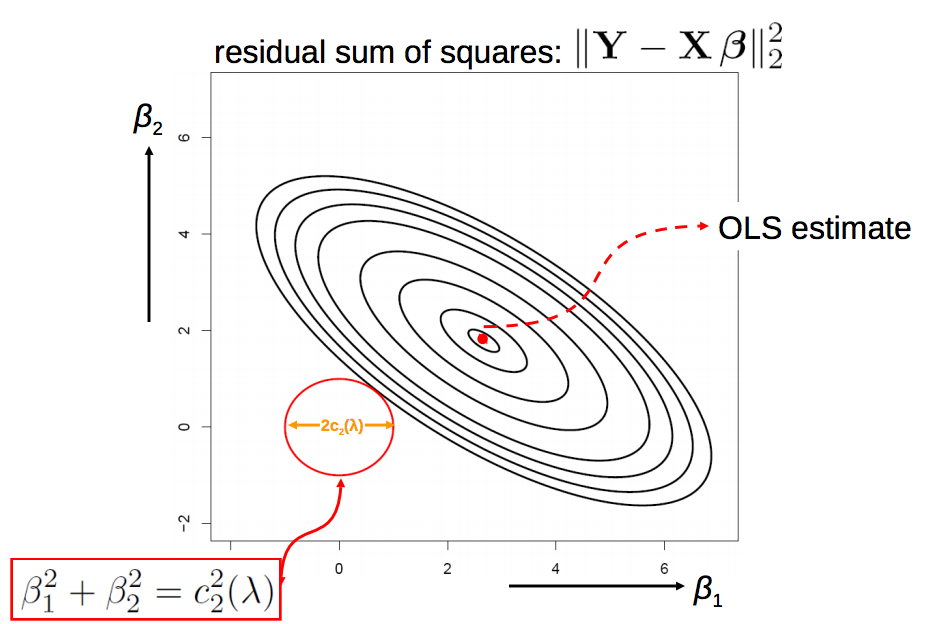
\includegraphics[width=0.9\linewidth]{img/geo1}
\end{figure}
}


\frame{
\frametitle{Geometric interpretation}
\begin{figure}
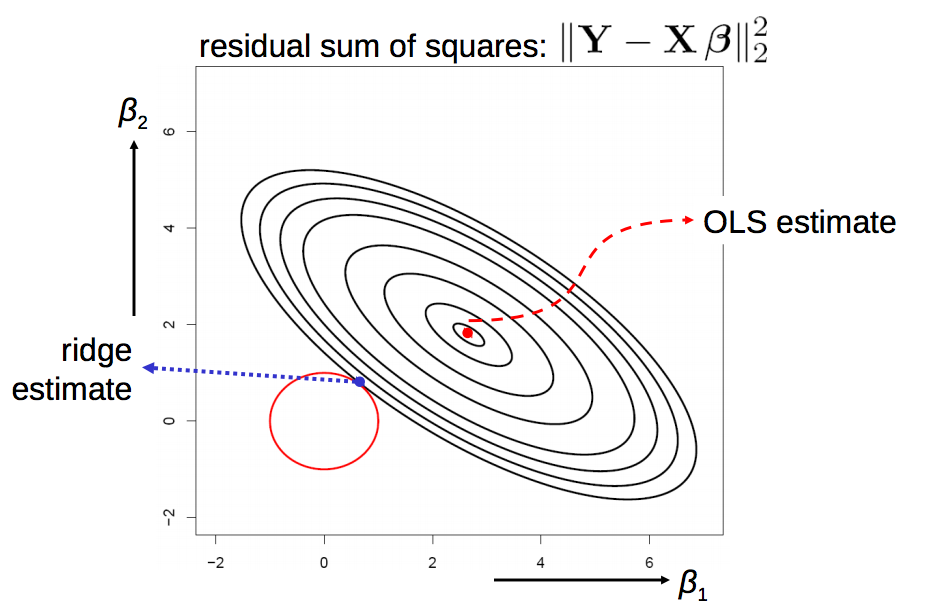
\includegraphics[width=0.9\linewidth]{img/geo2}
\end{figure}
}


\frame{
\frametitle{Choosing regularization parameter}
%Choise of $\lambda$ should balance the variance vs bias components of the mean squared error.
There is three main strategies to choose $\lambda$:
\begin{itemize}
\item Ridge trace
\item Effective degrees of freedom
\item Cross-validation
\end{itemize}
}


\frame{
\frametitle{Ridge trace}
Hoerl and Kennard (1970) \cite{hoerl+kennard1970} recommended the using of the \texttt{ridge trace}, a graphical display of all components of the vector $\phi_*$ against a range of values of $\lambda$.  Because $\lambda$ controls the amount of bias in the ridge estimate, the smallest value at which all coefficient traces are stabilized is chosen.
\begin{figure}
\includegraphics[width=0.6\linewidth]{img/ridgetrace}
\end{figure}
}

\frame{
\frametitle{The bias-variance trade-off}
The MSE of $\lambda$ is:
\begin{eqnarray*}
MSE(\lambda) &=& E[(\phi_*(\lambda)-\phi(\lambda))^\intercal(\phi_*(\lambda)-\phi(\lambda))] \\
&=& VAR(\lambda) + BIAS^2(\lambda)
\end{eqnarray*}
}

\frame{
\frametitle{Effective degrees of freedom}
}


\frame{
\frametitle{Cross-validation}
}

\frame{
\frametitle{Online Ridge regression}
Online RR is the online formulation of the regularized Least Squares method
and is based on the following equivalent formulation of the RR optimal solution.

\begin{eqnarray*}
\mathbf{\phi}_*&=&(\mathbf{X}^\intercal \mathbf{X}+\lambda
\mathbb{I})^{-1}\mathbf{X}^\intercal y \\
\mathbf{\phi}_* &=& \displaystyle \big (\sum_{t=1}^m
\mathbf{x}_t \mathbf{x}_t  ^\intercal + \lambda
\mathbb{I}\big)^{-1} \sum_{t=1}^m y_t
\mathbf{x}_t \\ \\
\mathbf{\phi}_*&=& \mathbf{A}^{-1}\mathbf{b}
\end{eqnarray*}

\noindent where $\mathbf{A}=\mathbf{X}^\intercal \mathbf{X} +\lambda
\mathbb{I}$ and $\mathbf{b}=\displaystyle  \sum_{t=1}^m y_t \mathbf{x}_t$.
}




\frame{
\frametitle{Proposal}

\begin{block}{Sliding window RR (SLRR)}
The method proposed consists of
a modification of RR considering a sliding window which contains only
the last $L$ samples. %and the new input $\mathbf{x}_t$, 
%i.e. $\{\mathbf{x}_i\}_{i=t-L+1}^{t-1}$. 
 
\[
\mathbf{X}(t) = 
\begin{bmatrix} 
\mathbf{x}_{t-L}^\intercal \\�\vdots \\ \mathbf{x}_t^\intercal
\end{bmatrix} \; , 
{\bf y}(t) = \begin{bmatrix} y_{t-L} \\�\vdots \\ y_t \end{bmatrix} \; .
\]
\end{block}

The optimal solution using a sliding windows is then:

\begin{problock}{SLRR solution}
\begin{eqnarray*}
\label{eq:optsolSLAAR}
{\bf \phi}(t)_*&=&({\bf X}(t)^\intercal{\bf X}(t)+\lambda
\mathbb{I})^{-1}{\bf X}(t)^\intercal{\bf y}(t) \\
{\bf \phi}(t)_*&=&{\bf A}(t)^{-1}{\bf b}(t) \\
\end{eqnarray*}
\end{problock}
}



\frame{
\frametitle{SLRR optimization}

It is worth noticing that the matrix $\mathbf{X}(t+1)$ is slightly
different from $\mathbf{X}(t)$:

\begin{equation} \label{eq:recform}
\mathbf{X}(t) = 
\begin{bmatrix} 
\mathbf{x}_{t-L}^\intercal \\�\vdots \\ \mathbf{x}_t^\intercal
\end{bmatrix} \qquad
\mathbf{X}(t+1) = 
\begin{bmatrix} \mathbf{x}_{t-L+1}^\intercal \\�\vdots \\
\mathbf{x}_{t+1}^\intercal
\end{bmatrix}
\end{equation}

Since $\mathbf{A}(t):=\mathbf{X}(t)^\intercal \mathbf{X}(t) +\lambda
\mathbb{I}$ then at time $t+1$:

\begin{eqnarray*}
\mathbf{A}(t+1)&=&\mathbf{X}(t+1)^\intercal
\mathbf{X}(t+1) +\lambda \mathbb{I} \\
&=&\mathbf{X}(t)^\intercal \mathbf{X}(t) + \mathbf{x}_{t+1}
\mathbf{x}_{t+1}^\intercal -
\mathbf{x}_{t-L} \mathbf{x}_{t-L}^\intercal +\lambda \mathbb{I} \\
&=& \mathbf{A}(t) + \mathbf{x}_{t+1}
\mathbf{x}_{t+1}^\intercal -
\mathbf{x}_{t-L} \mathbf{x}_{t-L}^\intercal
\end{eqnarray*}

}

\frame{
\frametitle{Matrix Inverse calculation}
It is required to get the inverse of the matrix $\mathbf{A}$ every new data
arrives, but we already calculated the matrix inverse of a matrix
slightly different.

The Sherman-Morrison-Woodbury formula allows to get the inverse of a
the matrix $\mathbf{A+uv^\intercal}$ if we already calculated the
inverse of $\mathbf{A}$ as follows:

\begin{equation}
(\mathbf{A+uv^\intercal})^{-1}=\mathbf{A}^{-1}-
\frac{\mathbf{A^{-1}uv^\intercal A^{-1}}}{\mathbf{1+v^\intercal A^{-1}u}}
\end{equation}

}

\frame{
\frametitle{Sherman-Morrison-Woodbury formula with two updates}
We need to get the inverse of the matrix
$\mathbf{A+uv^\intercal-wz^\intercal}$. In order to get the inverse we have
to solve the following equation:

\begin{eqnarray*}
(\mathbf{A+uv^\intercal-wz^\intercal)x} &=& \mathbf{b} \qquad
\mathbf{u,v,w,z,v} \in
\mathbb{R}^n \\
\mathbf{Ax + u\underbrace{\mathbf{v^\intercal x}}_{=:\xi} -
w\underbrace{\mathbf{z^\intercal
x}}_{=:\eta}} &=& \mathbf{b}
\end{eqnarray*}
Therefore we have to solve the system:
\[ \left[ 
\begin{array}{c:c:c} \mathbf{A} &  \mathbf{u} & \mathbf{-w}\\ \hdashline
\mathbf{v}^* & \mathbf{-1} & \mathbf{0} \\ \hdashline
\mathbf{z}^* & \mathbf{0} & \mathbf{-1}
\end{array} \right]
\left[
\begin{array}{c}
\mathbf{x} \\
\mathbf{\xi} \\
\mathbf{\eta}
\end{array}
\right]
=
\left[
\begin{array}{c}
\mathbf{b} \\
\mathbf{0} \\
\mathbf{0}
\end{array}
\right]
\]
}


\frame{
\frametitle{Solution}
Let $\alpha=\mathbf{v^\intercal A^{-1}u}$,
$\beta=\mathbf{v^\intercal A^{-1}w}$,
$\lambda=\mathbf{z^\intercal A^{-1}u}$,
$\delta=\mathbf{v^\intercal A^{-1}w}$ $\in \mathbb{R}$.
The factorization LU is:
\[  \setlength{\dashlinegap}{2pt} 
{\color{blue}
\left[
\begin{array}{c:c:c}
\mathbb{I} & 0 & 0 \\ \hdashline
\mathbf{v^* A^{-1}} & 1 & 0 \\ \hdashline
\mathbf{z^* A^{-1}} & \frac{\lambda}{1+\alpha} & 1 
\end{array}
\right]}
{\color{magenta}
\left[
\begin{array}{c:c:c}
\mathbf{A} & \mathbf{u} & \mathbf{-w} \\ \hdashline
0 & -1-\alpha & \beta \\ \hdashline
0 & 0 & -1+\delta-\frac{\lambda \beta}{1+\alpha} 
\end{array}
\right]}
\]
}

\frame{
\frametitle{Solution(2)}
First we solve the following system for $\mathbf{p,q,r}$:
\[  \setlength{\dashlinegap}{2pt} 
{\color{blue}
\left[
\begin{array}{c:c:c}
\mathbb{I} & 0 & 0 \\ \hdashline
\mathbf{v^* A^{-1}} & 1 & 0 \\ \hdashline
\mathbf{z^* A^{-1}} & \frac{\lambda}{1+\alpha} & 1 
\end{array}
\right]}
\left[
\begin{array}{c}
\mathbf{p} \\
\mathbf{q} \\
\mathbf{r} 
\end{array}
\right]
=
\left[
\begin{array}{c}
\mathbf{b} \\
\mathbf{0} \\
\mathbf{0} 
\end{array}
\right]
\]
and then:
\[
{\color{magenta}
\left[
\begin{array}{c:c:c}
\mathbf{A} & \mathbf{u} & \mathbf{-w} \\ \hdashline
0 & -1-\alpha & \beta \\ \hdashline
0 & 0 & -1+\delta-\frac{\lambda \beta}{1+\alpha} 
\end{array}
\right]}
\left[
\begin{array}{c}
\mathbf{x} \\
\mathbf{\xi} \\
\mathbf{\eta} 
\end{array}
\right]
=
\left[
\begin{array}{c}
\mathbf{p} \\
\mathbf{p} \\
\mathbf{r} 
\end{array}
\right]
\]
to get an expression for $\mathbf{x}$.
}

\frame{
\frametitle{Solution(3)}
We finally solve for $\mathbf{x}$:
\tiny
\[
\mathbf{x}=
\underbrace{
\left(
\mathbf{A}^{-1} - 
\mathbf{A}^{-1}\left[
\frac{1}{1+\alpha}\mathbf{uv^\intercal}-
\frac{c\beta}{1+\alpha}\mathbf{uz^\intercal}+
\frac{c\beta \lambda}{(1+\alpha)^2}\mathbf{uv^\intercal}+
c\mathbf{wz^\intercal} -
\frac{c\lambda}{1+\alpha}\mathbf{wv^\intercal}
\right]
\mathbf{A}^{-1}
\right)}_{({\color{red}\mathbf{A+uv^\intercal-wz^\intercal})^{-1}}} b
\]
}

\frame{
\frametitle{Accuumulated error}
\begin{figure}
\includegraphics[width=0.8\linewidth]{img/500}
\end{figure}
}

\frame{
\frametitle{Accuumulated error}
\begin{figure}
\includegraphics[width=0.8\linewidth]{img/1000}
\end{figure}
}

\frame{
\frametitle{Accuumulated error}
\begin{figure}
\includegraphics[width=0.8\linewidth]{img/2000}
\end{figure}
}
\frame{
\frametitle{Online Ridge regression algorithm}

\begin{algorithm}[H]
\begin{algorithmic}[1]
\REQUIRE $\,$ \\
$\{\mathbf{x}_1,\dots,\mathbf{x}_{m} \}$: $m$ input vectors \\
$\{y_1,\dots,y_{m} \}$: $m$ targets \\
$\lambda$: regularization parameter \\
\ENSURE  $\,$ \\
$\{f(\mathbf{x}_1),\dots,f(\mathbf{x}_{m}) \}$: model predictions \\
\STATE Initialize $\mathbf{A}=\lambda \mathbb{I}$
and $\mathbf{b}=0$
\FOR { $t = 1$ to $m$ }
	\STATE read new $\mathbf{x}_t$
	\STATE output prediction $f(\mathbf{x}_t) =  \mathbf{b}^\intercal \mathbf{A}^{-1}\mathbf{x}_t$
   	\STATE $\mathbf{A} = \mathbf{A} + \mathbf{x}_L
        \mathbf{x}_L^\intercal -\mathbf{x}_1 \mathbf{x}_1^\intercal $
   	\STATE Read new $y_t$
    	\STATE $\mathbf{b} = \mathbf{b} + y_t \mathbf{x}_t$
\ENDFOR

\end{algorithmic}
\caption{Ridge Regression}
\label{alg:RR}
\end{algorithm}
}

%\frame{
%\frametitle{Algorithm}
%\begin{algorithm}[ht]
%\begin{algorithmic}[1]
%\REQUIRE $\,$ \\
%$\{\mathbf{x}_1,\dots,\mathbf{x}_m \}$: $m$ input vectors \\
%$\{y_1,\dots,y_m \}$: $m$ targets \\
%$L$: sliding window size ($L<m$) \\
%$\lambda$: regularization parameter \\
%\ENSURE  $\,$ \\
%$\{f(\mathbf{x}_{L+1}),\dots,f(\mathbf{x}_m) \}$: model predictions \\
%\STATE Initialize $\mathbf{A}=\displaystyle \sum_{t=1}^L \mathbf{x}_t
%\mathbf{x}_t^\intercal + \lambda \mathbb{I}$
%and $\mathbf{b}=\displaystyle \sum_{t=1}^Ly_t \mathbf{x}_t$
%\FOR { $t = L+1$ to $m$ }
%        \STATE read new $\mathbf{x}_t$
%        \STATE output prediction $f(\mathbf{x}_t) =  \mathbf{b}^\intercal
%\mathbf{A}^{-1}\mathbf{x}_t$
%        \STATE $\mathbf{A} = \mathbf{A} + \mathbf{x}_t \mathbf{x}_t^\intercal-
%\mathbf{x}_{t-L-1} \mathbf{x}_{t-L-1}^\intercal  $
%        \STATE Read new $y_t$
%        \STATE $\mathbf{b} = \mathbf{b} + y_t \mathbf{x}_t - y_{t-L-1}\mathbf{x}_{t-L-1}$
%\ENDFOR
%
%\end{algorithmic}
%\caption{Recursive Ridge Regression}
%\label{alg:SLRR}
%\end{algorithm}
%}


\section{Model} \label{sec:proposal}
\frame{
\frametitle{Proposal}

\begin{itemize}
\item As the cointegration factors and vectors don't vary much at every step, they are recalculated every certain amount of time defined as a parameter.
\item The number of cointegration vectors is set as a parameter.
\end{itemize}
}

\frame{
\frametitle{Proposal algorithm}

\begin{algorithm}[H]
\algsetup{linenosize=\tiny}
\scriptsize
\begin{algorithmic}[1]
\REQUIRE $\,$ \\
\begin{tabular}{ll}
$\color{red}\{\mathbf{p}_1,\dots,\mathbf{p}_N \}$: $N$ price vectors &
$\color{red}L$: sliding window size ($L<N$) \\
$\color{red}\lambda$: regularization parameter &
$\color{red}\mu$: cointegration vector update step \\
$\color{red}r$: number of cointegration vectors &
$\color{red}nlag$: number of past values 
\end{tabular}\\
\ENSURE  $\,$ \\
$\{f(\mathbf{p}_{L+1}),\dots,f(\mathbf{p}_N) \}$: model predictions\\
\STATE Initialize $\mathbf{A}=\lambda \mathbb{I}$ 
and $\mathbf{b}=0$
\FOR { $t =1$ to $N-L$ }
	\IF {t == 1 \OR \NOT mod(t,$\mu$)}
	\STATE{$jvectors = {\color{blue}\text{getJohansen}}(r, \{\mathbf{p}_t,\dots,\mathbf{p}_{t+L} \})$}
	\STATE{$[\mathbf{X} \quad \mathbf{Y}] = {\color{blue}\text{createMatrix}}(jvectors,\{\mathbf{p}_t,\dots,\mathbf{p}_{t+L} \},nlag)$}
	\STATE{$\mathbf{A}=\mathbf{X}^\intercal \mathbf{X} + \lambda \mathbb{I}$ \quad $\mathbf{b}=\mathbf{X}^\intercal \mathbf{Y}$}
	\ELSE
        \STATE $[\mathbf{x}_{L} \quad \mathbf{x}_{1} \quad \mathbf{y}_{L} \quad \mathbf{y}_{1}] =
        {\color{blue}\text{createVectors}}(\mathbf{X},\mathbf{Y},\mathbf{p}_{t+L},nlag)$
        \STATE output prediction $f(\mathbf{x}_t) =  \mathbf{b}^\intercal
\mathbf{A}^{-1}\mathbf{x}_{L}$
        \STATE $\mathbf{A} = \mathbf{A} + \mathbf{x}_{L} \mathbf{x}_{L}^\intercal-
\mathbf{x}_{1} \mathbf{x}_{1}^\intercal  $
        \STATE Read new $y_t$
        \STATE $\mathbf{b} = \mathbf{b} + y_{L} \mathbf{x}_{L} - y_{1}\mathbf{x}_{1}$
        \ENDIF
\ENDFOR

\end{algorithmic}
\caption{SLRR}
\label{alg:RR}
\end{algorithm}
}


%\frame{
%\frametitle{Original algorithm modifications}
%
%\begin{itemize}
%\item Only a sliding windows of data is used instead of all past data,
%which would increase the size of every new input. This was done in order
%to compare execution times.
%\item Cointegration vectors and factors are calculated every time step.
%\item The number of cointegration vectors are determined by the Johansen method.
%\end{itemize}
%}

\section{Experiments}
\frame{
\frametitle{Data}

The data used in this article was obtained from Dukascopy historical
bid and ask prices. We used currency prices every
minute from the 2nd of January 2012 to the 18th of November 2013,
which were 987.454 inputs.

\begin{figure}
\includegraphics[width=0.65\linewidth]{img/data}
\end{figure}

}


\frame{
\frametitle{Setting Lags and window size}
AIC for different combinations of Lags and window sizes were done, the best AIC values are shown un a red scale.

\begin{figure}
\includegraphics[width=0.7\linewidth]{img/AIC_AUDSGD}
\caption{AIC: Lags vs Sliding window size for AUDSGD}
\end{figure}

}


\frame{
\frametitle{Setting Lags and window size}
\begin{figure}[H]
\centering
\begin{tabular}{cc}

\subfloat[AUDSGD]{
    \includegraphics[width=0.3\linewidth]{img/AIC_AUDSGD}
    \label{fig:currency1}
}
&
\subfloat[NZDJPY]{
    \includegraphics[width=0.3\linewidth]{img/AIC_NZDJPY}
    \label{fig:currency2}
}
\\
\subfloat[AUDNZD]{
    \includegraphics[width=0.3\linewidth]{img/AIC_AUDNZD}
    \label{fig:currency3}
}
&
\subfloat[CHFJPY]{
    \includegraphics[width=0.3\linewidth]{img/AIC_CHFJPY}
    \label{fig:currency4}
}

\end{tabular}
\caption{AIC: Lags vs Sliding window size}
\label{fig:lagoptimization}
\end{figure}

}
\frame{
\frametitle{lambda optimization}
\begin{figure}
\includegraphics[width=0.8\linewidth]{img/gamma}
\end{figure}
}
\frame{
\frametitle{Time optimization}
\begin{center}
\begin{tabular}{cccc}
Method,&N&Jstep&Time \\ \hline
SLECM&2000&- &0.629035 \\
SLAAR&2000&100&0.066171
\end{tabular}
\end{center}
}

\bibliographystyle{IEEEtran}
\bibliography{reference}

\end{document}
